%%%%%\section{Array computing and curve plotting}

\begin{Problem}{\textbf{Fill arrays; loop version}} \label{prob51}
%\addcontentsline{toc}{section}{Exercise 5.1: Fill arrays; loop version - \texttt{fill\_arrays\_loop.py}}

\noindent We study the function
\begin{equation*}
f(x) = \ln(x).
\end{equation*}
We want to fill two arrays \pythoninline{x} and \pythoninline{y} with the values of $x$ and $f(x)$,
respectively. Use $101$ uniformly spaced $x$ values in the interval $[1, 10]$.
First create arrays \pythoninline{x} and \pythoninline{y} with the correct length, containing
all zeros. Then compute and fill in each element in
\pythoninline{x} and \pythoninline{y} with a \pythoninline{for} loop.

Filename: \texttt{fill\_log\_arrays\_loop.py}
\end{Problem}

\begin{Problem}{\textbf{Fill arrays; vectorized version}}
%\addcontentsline{toc}{section}{Exercise 5.2: Fill arrays; vectorized version - \texttt{fill\_arrays\_vectorized.py}}

\noindent Vectorize the code in Problem \ref{prob51} by creating the $x$ values using the
\pythoninline{linspace} function from the \pythoninline{numpy} package and evaluating
$f(x)$ with an array argument. Since the calculation should be vectorized, you should not
use any form of loop in the code.

Filename: \texttt{fill\_log\_arrays\_vectorized.py}
\end{Problem}



\begin{Problem}{\textbf{Plot the population growth}}
%\addcontentsline{toc}{section}{Exercise 5.3: Plot the population growth - \texttt{pop\_plot.py}}

\noindent Again, we're considering a population undergoing logistic growth. The number of
individuals in the population is given by
\begin{equation*}
N(t, k, B, C) = \frac{B}{1 + C \exp{-kt}}.
\end{equation*}
Plot this function for $t \in [0, 48]$ with a carrying capacity $B = 50 000$,
$C = 9$ from the initial condition that we have $5 000$ individuals at $t = 0$
and a steepeness of $k = 0.2$.

Filename: \texttt{population\_plot.py}
\end{Problem}

\begin{Problem}{\textbf{Oscillating spring}}

\noindent A rock of mass $m$ is hung from a spring, and pulled down a length $A$. When
released, the rock will oscillate up and down with a
vertical position given by
\[
y(t) = A e^{-\gamma t}\cos\left(\sqrt{\frac{k}{m}}t\right),
\]

Here, $y$ is the vertical position of the rock, $k$ is the spring
constant, and $\gamma$ is a friction coefficient representing
air resistance. Set $k = 4$ kg s$^{-2}$ and $\gamma = 0.15$ s$^{-1}$,
$m = 9$ kg, and $A = 0.3$ m.
\paragraph{a)} Create arrays \pythoninline{t_array} and
\pythoninline{y_array} of size 101, both initially filled with zeros.
Use a \pythoninline{for} loop to fill them with time values in the range from 0 to 25 seconds, and the
corresponding $y(t)$ values.
\paragraph{b)} Vectorize your program by using the NumPy's \pythoninline{linspace}
function to generate the \pythoninline{t_array}, and
send it into a function \pythoninline{y(t)} to generate the \pythoninline{y_array}. Your program should now be free of
for loops.
\paragraph{c)} Plot the position of the rock against time in the given time
interval. Use the arrays from both exercise a) and b), and confirm that they
give the same result. Put the correct units on both axes.

Filename: \texttt{oscillating\_spring.py}
\end{Problem}

\begin{Problem}{\textbf{Plot Stirling's approximation}}
%\addcontentsline{toc}{section}{Exercise 5.4: Plot Stirling's approximation - \texttt{stirling\_plot.py}}

\noindent Stirling's approximation is
\begin{equation*}
\ln (x!) \approx x\ln x - x.
\end{equation*}
\paragraph{a)} Make two functions \pythoninline{stirling(x)} and \pythoninline{exact(x)},
returning Stirling's approximation and the exact value of $\ln (x!)$, respectively.
Plot both the approximation and the exact curve in the same figure.

\emph{Hint: To implement a vectorized version of the \pythoninline{exact} function,
you can use scipy.special.gamma(x). This function is a ``generalized factorial''
which can find the ``factorial'' of float numbers. It works such that
$n! = \mathrm{gamma}(n + 1)$. You can also just consider integer values and plot
the value of $\ln (x!)$ for each integer $x$ in the interval you're considering.
Keep in mind that \pythoninline{math.factorial} is not vectorized.}

\paragraph{b)} Use a \pythoninline{while} loop and find the minimal value of $x$ for
the relative error to be less than $0.1\%$.

\emph{Hint: Relative error is given as $(a - \tilde{a})/a$, where $a$ is the exact
value and $\tilde{a}$ is the approximation. Also, do not start with $x$ smaller
than or equal to $1$, why?}

Filename: \texttt{stirling\_plot.py}
\end{Problem}


\begin{Problem}{\textbf{Plotting roots of a complex number}}

\noindent The $n$'th roots of a complex number $z = r e^{i \theta}$ can be found by
\begin{equation*}
    \omega_k = \sqrt[^n]{z} = \sqrt[^n]{r} e^{\mathrm{i \frac{\theta + 2 \pi k}{n}}},
\end{equation*}
for $k = 0, 1, ..., n-1$. The roots can be rewritten to separate the real component $x_k$ and the imaginary component $y_k$, such that $\omega_k = x_k + i y_k$. Through the relation between the exponential function and the sine functions we get
\begin{equation*}
    x_k = r^{\frac{1}{n}} \cos{\frac{\theta + 2 \pi k}{n}}
\end{equation*}
and
\begin{equation*}
    y_k = r^{\frac{1}{n}} \sin{\frac{\theta + 2 \pi k}{n}} ,
\end{equation*}
for $k = 0, 1, ..., n-1$.

\paragraph{a)}
Write a function that takes the angle $\theta$, the radius $r$ and the degree $n$ of the roots as parameters. The function should calculate and return  all of the $n$'th roots of a complex number $r e^{i \theta}$, as two lists or arrays corresponding to the real part $x = x_0, x_1, ..., x_{n-1}$ and the complex part $y =y_0, y_1, ..., y_{n-1}$ of the roots. An example of a function call on the function you will write is given below.
\begin{python}
x, y = roots(r, theta, n)
\end{python}

\paragraph{b)}
Consider the complex number $z = 10^{-4}e^{i 2 \pi}$. Use the function from a) to get all the roots of order $n = 6$, $n = 12$ and $n = 24$. Plot the roots as points, and plot all the three orders of roots in the same plot. Label the different orders of roots. And example of code for plotting the roots of order $n = 6$ is given below.
\begin{python}
plt.plot(x_n_6, y_n_6, "o", label="n = 6")
\end{python}
Filename: \texttt{roots.py}
\end{Problem}


\begin{Problem}{\textbf{Fermi-Dirac distribution}} \label{prob55}
%\addcontentsline{toc}{section}{Exercise 5.5: Fermi-Dirac distribution - \texttt{Fermi\_Dirac.py}}

\noindent The Fermi-Dirac distribution says something about the probability of an energy
state being occupied by a particle, or more precisely a fermion, e.g. an electron.
It is a function of energy and temperature given by
\begin{equation}
f(E, T) = \frac{1}{1 + e^{(E - \mu)/kT}},
\end{equation}
where $E$ is energy, $T$ is temperature, $k$ is Boltzmann's constant and $\mu$ is
the so-called chemical potential. Use $k = 8.6 \cdot 10^{-5}\mathrm{eVK^{-1}}$ and
$\mu = 4.74$eV and make a program that visualizes the Fermi-Dirac distribution on
the interval $E \in [0, 10]$eV when $T = 0.1$K. (eV is a unit of energy, $1\mathrm{eV}
= 1.6\cdot 10^{-19}\mathrm{J}$.)

Filename: \texttt{Fermi\_Dirac.py}
\end{Problem}

\begin{Problem}{\textbf{Animate the temperature dependence of the Fermi-Dirac distribution}}
%\addcontentsline{toc}{section}{Exercise 5.6: Animate the temperature dependence of the Fermi-Dirac distribution - \texttt{Fermi\_Dirac\_movie.py}}

\noindent Make an animation of the Fermi-Dirac distribution $f(E, T)$ from Problem \ref{prob55}
We're interested in studying how the distribution changes when we raise the temperature.
Plot $f$ as a function of $E$ on $[0, 10]$ for a set of temperatures
$T \in [0.1, 3 \cdot 10^{4}]$. Also make an animated GIF file. Remember
to label your axes and include a legend to show the value of the temperature.

\emph{Hint: A suitable resolution can be $1 000$ intervals ($1 001$ points) along
the $E$ axis,  $60$ intervals ($61$ points) in temperature, and $6$ frames per
second in the animated GIF file. Use the recipe in Section 5.3.4 and remember to
remove the family of old plot files in the beginning of the program.}

Filename: \texttt{Fermi\_Dirac\_movie.py}
\end{Problem}

\begin{Problem}{\textbf{Bump functions}}

\noindent Consider the function
\begin{equation*}
   f(x)=\begin{cases}
       ke^{-\frac{1}{1-x^2}} & -1 < x < 1 \\
       0 & otherwise.
   \end{cases}
\end{equation*}

\paragraph{a)}
Plot the function with $k=1$ on the interval $-2 \leq x \leq 2$ by implementing
a vectorized version in your program.

\paragraph{b)}
Animate the function on the same interval as above when $k$ decreases from
1 to 0.

Filename: \texttt{bump.py}
\end{Problem}

\begin{Problem}{\textbf{Band structure of solids}}
%\addcontentsline{toc}{section}{Exercise 5.7: Band structure of solids - \texttt{band\_structure.py}}

\noindent Electrons in solids are waves. These waves have different wave lengths $\lambda$.
Often, waves are characterised by their wave number $k = 2\pi/\lambda$, and the
wave number is associated with the energy of the electron. The energies of electrons
in solids have a band structure, i.e., there are different bands of energies
separated by a band gap.

The file \texttt{bands.txt} contains $k$-values and corresponding energies for
the three first bands of a solid. Have your program read the values for $k$ and
the energies and plot the energy bands as functions of $k$ in the same figure.
You will see that some energies can never be obtained by electrons in the solids.
These areas of non-allowed energies are called the band gaps.

Filename: \texttt{band\_structure.py}
\end{Problem}


\begin{Problem}{\textbf{Half-wave rectifier vectorized}}
%\addcontentsline{toc}{section}{Exercise 5.8: Half-wave rectifier vectorized - \texttt{half\_wave\_vec.py}}

\noindent In Problem \ref{prob34}, we implemented a function illustrating a sine signal after it
had passed through a half-wave rectifier. Vectorize this function and plot $f(x)$
for $x \in [0, 10\pi]$.

\emph{Hint: The \pythoninline{numpy.where(condition, x1, x2)} function returns an
array of the same length as \pythoninline{condition}, whose element number
\pythoninline{i} equals \pythoninline{x1[i]} if \pythoninline{condition} is \pythoninline{True},
and \pythoninline{x2[i]} otherwise.}

Filename: \texttt{half\_wave\_vec.py}
\end{Problem}


\begin{Problem}{\textbf{Singularity plot}}

\noindent In this problem we consider the function
\begin{equation*}
    f(r,\theta)=\left(e^{\frac{1}{r}\cos{\theta}}\cos\left(-\frac{1}{r}\sin{\theta}\right),
    			-e^{\frac{1}{r}} \sin\left(-\frac{1}{r}\sin{\theta}\right)\right)
\end{equation*}
with $0.01\leq r \leq 1$ and $0\leq \theta \leq 2\pi$. Create arrays of $r$ and
$\theta$ values on the unit circle centered at the origin with $n$ uniformly
spaced values. Fix axes between
-0.5 and 0.5 for $x$ and $y$ and visualize the function for $n=10,50,100,500$.
You can use the following to generate the correct values for $r$ and $\theta$:
\begin{python}
theta = np.linspace(0,2*np.pi,100)
r = np.linspace(0.01,1,100)
r, theta = np.meshgrid(r,theta)
\end{python}

\begin{remark}
If we had an ideal computer that could calculate every value in an interval and
plot it, then the image we have plotted would touch every single value in the
plane, except for at most one! In our program we have $0.01<r<1$. The remarkable
thing is that the same is true if we replace the inequality with $0<r<\epsilon$
for any $\epsilon > 0$. Not only that, but all those points are hit an infinite
number of times!
\end{remark}

Filename: \texttt{ess\_sing.py}
\end{Problem}

\begin{Problem}{\textbf{Approximate $|x|$}}

\noindent The absolute value $f(x)=|x|$ can be written as a sum
\begin{equation*}
	f(x)=\frac{\pi}{2}-\frac{4}{\pi} \sum_{n=1}^\infty \frac{\cos((2n-1)x)}{(2n-1)^2}.
\end{equation*}
Write a program that calculates the first $N$ terms for $N=1,2,3,4$ and plots it against
the exact function. Let the x-axis be $[-\pi,\pi]$ with a suitable y-axis.

Filename: \texttt{approx\_abs.py}
\end{Problem}

\begin{Problem}{\textbf{Plotting graphs}}

\noindent A graph is a collection of lines and points in the plane
such that each line connects two points. In this exercise we will create functions for
plotting graphs on a set of points.

\paragraph{a)}
Make a function \pythoninline{plot_line(p1,p2)} that takes two points as input arguments
and plots the line between them. The two input arguments should be lists or tuples specifying
$x$- and $y$-coordinates, i.e. \pythoninline{p1 = (x1,y1)}. Demonstrate that the function works by plotting a vertical and a horizontal line.

\paragraph{b)}
A complete graph is a graph such that any two points has a line that connects them. Make a function that takes a list of points and plots the complete graph on those points. To verify that the
function works, first choose the four corners of the square ($(0,0),(1,0),(0,1),(1,1)$)
and then the points $(1,0), (\alpha,\alpha), (0,1), (-\alpha,\alpha),
(-1,0), (-\alpha,-\alpha),(0,-1), (\alpha,-\alpha)$, with $\alpha=\sqrt{2}/2$. The resulting
complete graphs should look like the ones in Figure \ref{fig:graphs}.

Hint: Modify the \pythoninline{plot_line} function from 5.14 a) so that it only calls
\pythoninline{plot()} but not \pythoninline{show()}. The complete graph can then be drawn by
looping over the points and calling \pythoninline{plot_line} for each pair, and finally calling
\pythoninline{show()} after the loop.

Filename: \texttt{graph1.py}
\end{Problem}

\begin{figure}
    \centerline{
    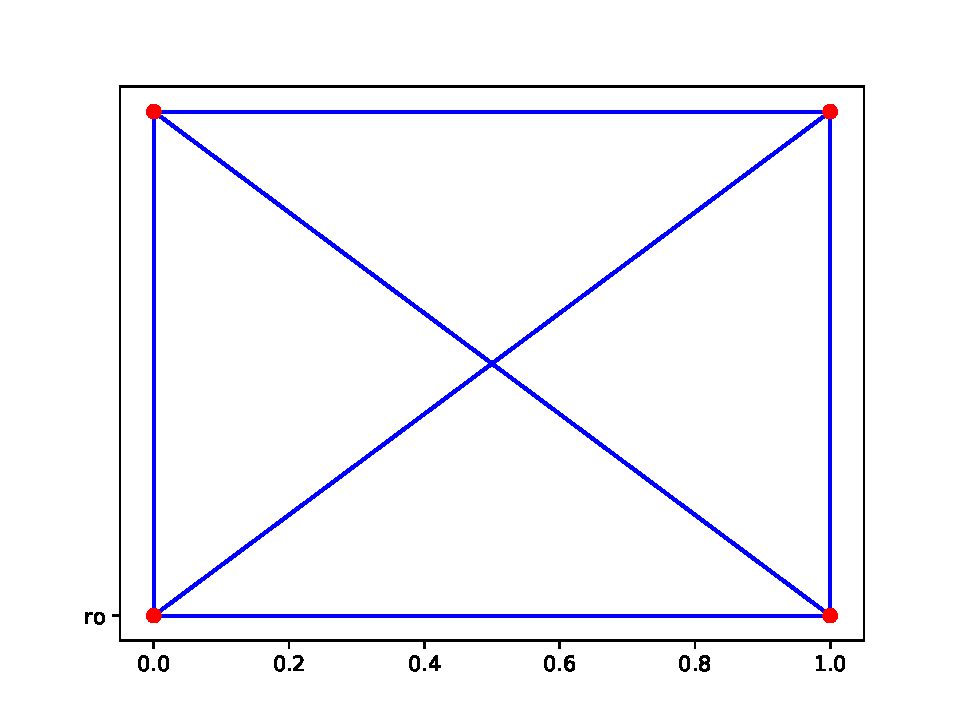
\includegraphics[width=0.45\linewidth]{./figs/square.pdf}
    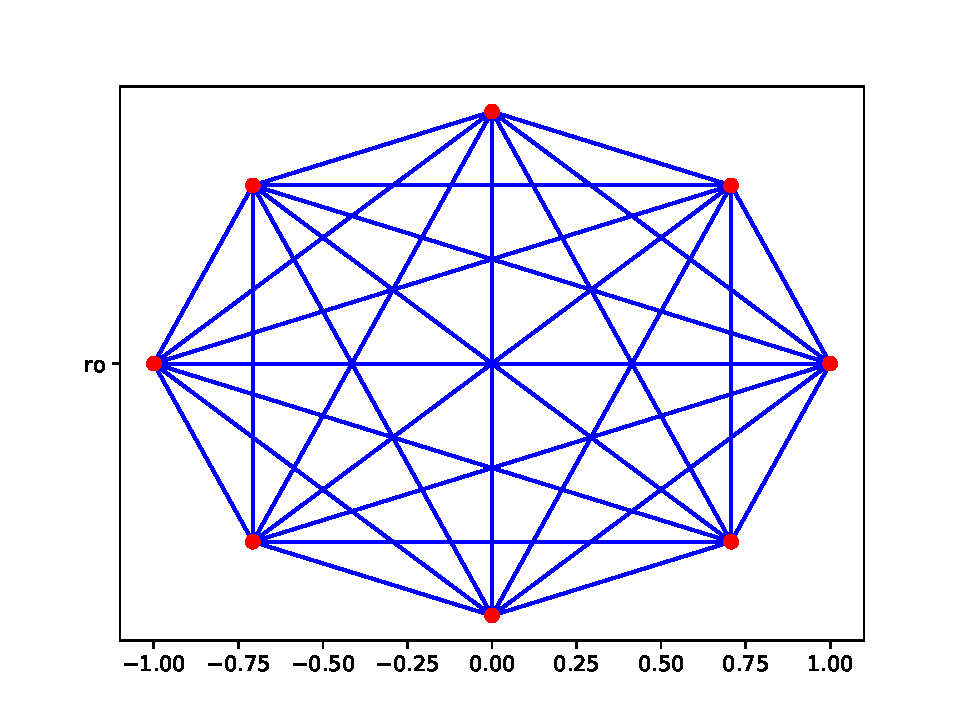
\includegraphics[width=0.45\linewidth]{./figs/circle.pdf}}
    \caption{Examples of complete graphs from Problem 5.14 b). The left shows the graph on the
    corners of the unit square, the right is the graph for eight equally spaced points on a circle.}
    \label{fig:graphs}
\end{figure}


\begin{Problem}{\textbf{Plotting graphs}}

\noindent Given a natural number $n$, make a function that plots the following graph:
\begin{itemize}
    \item Two vertical rows with $n$ points should be placed side by side.
    \item Each point on the left side should have a line to every point on the
    right side and vice versa.
    \item No two points on the same side should be connected by a single line.
\end{itemize}
Filename: \texttt{graph2.py}
\end{Problem}


\begin{Problem}{\textbf{Inefficiency of primality checker}}

\noindent Consider the program from Problem \ref{prime}. Use the \pythoninline{timeit} module and run the
program to find the time it takes to find a factorization of an $n$ digit number. Plot the time against
the number of digits for the numbers in the file \texttt{prime\_check.dat}.
You can use the following code to time the function for different numbers:
\begin{python}
str1 = "f(" + str(n) + ")"
str2= "g(" + str(n) + ")"
N = 100
time1 = timeit.timeit(str1, 'from __main__ import f',number=N)
time2 = timeit.timeit(str2, 'from __main__ import g',number=N)
\end{python}

Filename: \texttt{prime\_ineff.py}
\end{Problem}

\begin{Problem}{\textbf{Animating a cycloid}}

\noindent One may create a curve by placing a circle on the $x$-axis, fixing a point on the circle,
and then drawing the trace of the point as the circle is rolling. The resulting
curve is called a cycloid. In mathematical language it is given as
\begin{equation*}
    r(\theta) =[R(\theta-\sin\theta), R(1-\cos \theta)]
\end{equation*}
where $R$ is the radius of the rotating circle and $\theta$ is the angle starting
at 0 and increasing.

\paragraph{a)}
Animate the cycloid as a function of $\theta$ starting at 0, ending at 15. Draw
a point at the end of the cycloid that varies with the animation.

\emph{Hint: A point can be added through a new plot using for example}
\newline
\pythoninline{point, = axes.plot([],[],'o')}

\emph{and updating during the animation.}

\paragraph{b)}
Add the rolling circle defining the cycloid to the plot. You may use that at a given
time $\theta$, the circle is given as $s(\theta)=(R\cdot\theta + \cos\theta, R + \sin\theta)$.

Filename: \texttt{cycloid.py}
\end{Problem}

\begin{Problem}{\textbf{Calibration curve}}

\noindent
A tool in chemical analysis for measuring the concentration of a substance in a sample (e.g. blood or urine), is making a calibration curve. Solutions with known concentrations of a substance (standard solutions) are measured. The X-axis is the concentrations of the standard solutions, and the Y-axis is for the measured intensity of these solutions. The concentration of the substance in the sample can then be determined using an equation that best describes the calibration curve. This equation is determined using linear regression.

In Python, you can use the \pythoninline{numpy} module to obtain a linear regression. How to do this will be shown.

Assume that you have made five standard solutions with concentrations of 10, 20, 30, 40 and 50 mg/L of the substance you wish to test for. You have used equipment that detects this substance, and noted down the intensity for each of your standard samples. The code below shows how the linear regression can be performed.
\begin{python}
# standard concentrations and height of their signals
I_stand = [9.19, 19.8, 27.0, 34.7, 44.9]
conc_stand = [10, 20, 30, 40, 50]

# linear regression
fit = np.poly1d(np.polyfit(conc_stand, I_stand, 1))
conc_curve = np.linspace(0, 60, 100)
signal_curve = fit(conc_curve)
\end{python}

\paragraph{a)}
Plot the calibration curve as a line, and plot the intensities of the calibration solutions as points on top of the calibration curve.

\paragraph{}
\noindent
The function created in the code above, \pythoninline{fit(x)}, is now a linear function on the form $f(x) = a x + b = y$, where $x$ corresponds to the concentration and $y$ will correspond to the intensity of the signal at the given concentration.

\paragraph{b)}
Determine $a$ and $b$ by using \pythoninline{fit(x)} and use these to implement an inverse function of $f(x)$ such that $g(y) = x$. Use your function to calculate the concentration of three different samples of the same unknown compound. The intensities of the compound of the samples are given below.
\begin{python}
I_unknown = np.array([19.9, 20.1, 19.8])
\end{python}
Print out the mean value, with the uncertainty ($\overline{x} \pm s_N$), of the samples of the unknown compound. You may use \pythoninline{np.mean} and \pythoninline{np.std} to find the mean value and the uncertainty.

Filename: \texttt{calibration.py}
\end{Problem}
